\documentclass{article}
\usepackage{fancyhdr}
\usepackage{extramarks}
\usepackage{amsmath}
\usepackage{amsthm}
\usepackage{amsfonts}
\usepackage{tikz}
\usepackage[plain]{algorithm}
\usepackage{algpseudocode}

\begin{document}
\author{Chuan Lu}
\title{MATH:7830 Homework 1}
\maketitle


\begin{figure}[h]
\centering
\vbox{
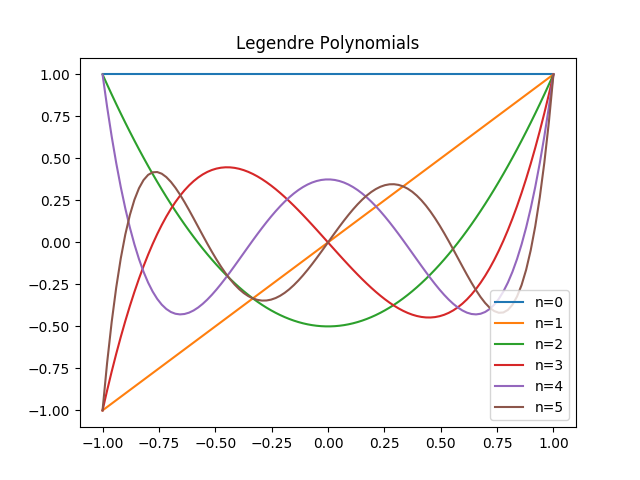
\includegraphics[scale=0.35]{Images/legendre.png}
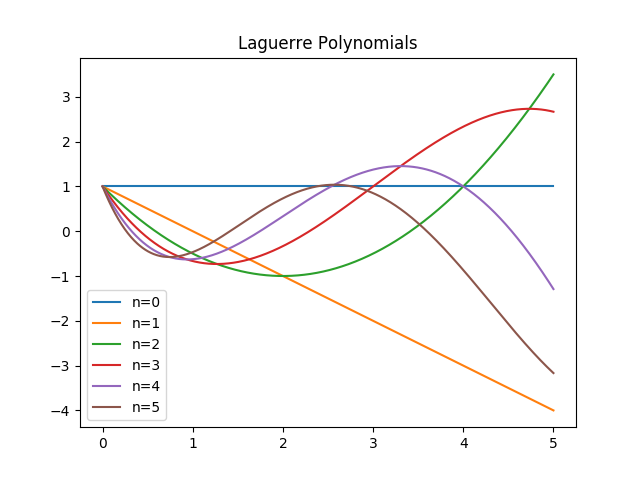
\includegraphics[scale=0.35]{Images/laguerre.png}
} 
\vbox{
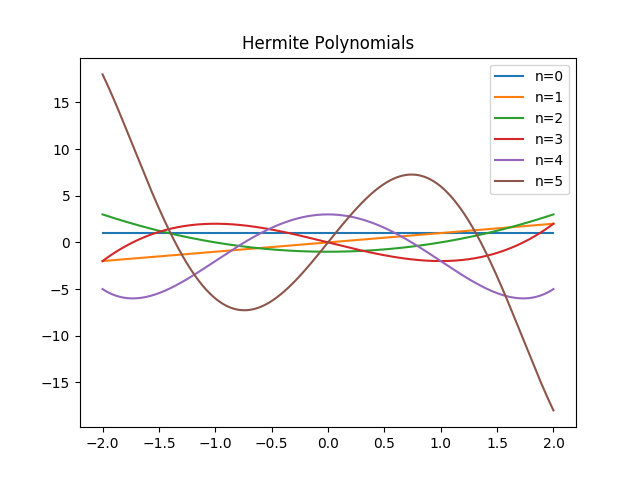
\includegraphics[scale=0.35]{Images/hermite.png}
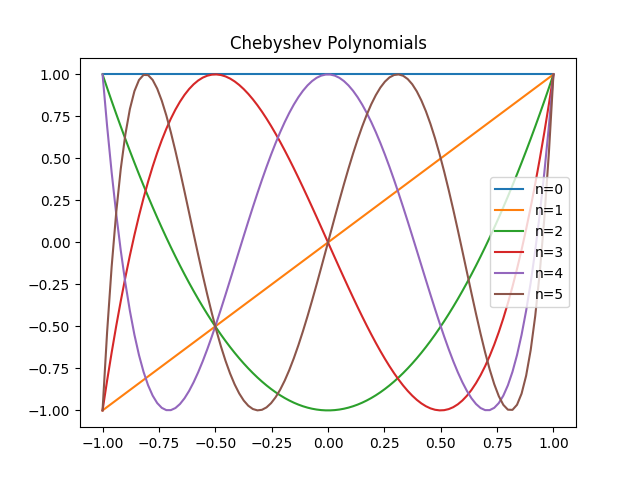
\includegraphics[scale=0.35]{Images/chebyshev.png}
}
\caption{Legendre, Laguerre, Hermite and Chebyshev polynomials up to order 5.}
\end{figure}

\end{document}